\section{LU分解}
\label{sec:ls-lu}

一般非奇异方阵没有对称性或正定性可以利用，最基本的求解方式是第~\ref{sec:ls-gaussian-elimination}节的Gauss消元。本节把消元过程记录成两个三角因子，使求解化为两次三角代入；行交换用来避开零主元和过小的主元，因子一旦算出，换右端时可以直接复用。

\subsection{主要思想}
设$\bm A\in\mathbb R^{d\times d}$非奇异，$\bm b\in\mathbb R^d$，要求$\bm A\bm x=\bm b$的唯一精确解$\bm x_\star$。假设已经得到\term{LU分解}
\begin{equation}
 \bm P\bm A=\bm L\bm U,
 \label{eq:ls-palu}
\end{equation}
其中$\bm P$是置换矩阵，$\bm L$是单位下三角矩阵（对角元都为$1$），$\bm U$是非奇异上三角矩阵。这三个矩阵怎样由Gauss消元算出，留到下一小节；本小节说明有了分解以后怎样求出$\bm x$。

把方程$\bm A\bm x=\bm b$两边左乘$\bm P$，得$\bm P\bm A\bm x=\bm P\bm b$。左乘置换矩阵只是重排方程的先后次序，不改变解。记$\bm c=\bm P\bm b$，代入分解，方程成为
\[
 \bm L\bm U\bm x=\bm c .
\]
令$\bm y=\bm U\bm x$，它又写成$\bm L\bm y=\bm c$。所以求解分两步：先由$\bm L\bm y=\bm c$求出$\bm y$，再由$\bm U\bm x=\bm y$求出$\bm x$。两个方程的系数矩阵都是三角矩阵，可以逐个分量求解。

\paragraph{前代：求解$\bm L\bm y=\bm c$}
为了让公式也能用于对角元不为$1$的下三角矩阵（例如第~\ref{sec:ls-cholesky}节的Cholesky因子），先设$\bm L$是对角元都不为零的一般下三角矩阵。按行写出$\bm L\bm y=\bm c$：
\[
 \begin{aligned}
 l_{1,1}y_1&=c_1,\\
 l_{2,1}y_1+l_{2,2}y_2&=c_2,\\
 &\ \,\vdots\\
 l_{d,1}y_1+l_{d,2}y_2+\cdots+l_{d,d}y_d&=c_d .
 \end{aligned}
\]
第一个方程只含$y_1$，得$y_1=c_1/l_{1,1}$。第二个方程中$y_1$已经求出，移项后得$y_2=(c_2-l_{2,1}y_1)/l_{2,2}$。一般地，第$i$个方程是
\[
 \sum_{j<i}l_{i,j}y_j+l_{i,i}y_i=c_i ,
\]
其中$y_1,\ldots,y_{i-1}$已由前面的方程求出。把它们移到右边，再除以$l_{i,i}$，得
\begin{equation}
 y_i=\frac{c_i-\sum_{j<i}l_{i,j}y_j}{l_{i,i}}\qquad(i=1,2,\ldots,d).
 \label{eq:ls-forward-substitution}
\end{equation}
按$i=1,2,\ldots,d$的顺序计算，右侧用到的都是已经算出的分量。这种求解顺序称为\term{前代}；只要对角元都不为零，它逐个唯一地给出解。LU中$l_{i,i}=1$，公式化为$y_i=c_i-\sum_{j<i}l_{i,j}y_j$，不需要除法。

\paragraph{回代：求解$\bm U\bm x=\bm y$}
$\bm U$非奇异，它的行列式是对角元之积，所以对角元都不为零。按行写出$\bm U\bm x=\bm y$：
\[
 \begin{aligned}
 u_{1,1}x_1+u_{1,2}x_2+\cdots+u_{1,d}x_d&=y_1,\\
 &\ \,\vdots\\
 u_{d-1,d-1}x_{d-1}+u_{d-1,d}x_d&=y_{d-1},\\
 u_{d,d}x_d&=y_d .
 \end{aligned}
\]
这次最后一个方程只含$x_d$，得$x_d=y_d/u_{d,d}$。倒数第二个方程中$x_d$已经求出，得$x_{d-1}=(y_{d-1}-u_{d-1,d}x_d)/u_{d-1,d-1}$。一般地，第$i$个方程是
\[
 u_{i,i}x_i+\sum_{j>i}u_{i,j}x_j=y_i ,
\]
其中$x_{i+1},\ldots,x_d$已由后面的方程求出，移项后除以$u_{i,i}$，得
\begin{equation}
 x_i=\frac{y_i-\sum_{j>i}u_{i,j}x_j}{u_{i,i}}\qquad(i=d,d-1,\ldots,1).
 \label{eq:ls-back-substitution}
\end{equation}
按$i=d,d-1,\ldots,1$的顺序计算，这种求解顺序称为\term{回代}。

图~\ref{fig:ls-triangular-substitution-order}对比了两种顺序：前代自上而下，每个分量只依赖它上方已求出的分量；回代自下而上，依赖关系正好反过来。后面各节遇到三角方程时，直接调用前代和回代。分解只依赖$\bm A$，换一个右端只需重新做这两次代入。

\begin{figure}[!htb]
  \centering
  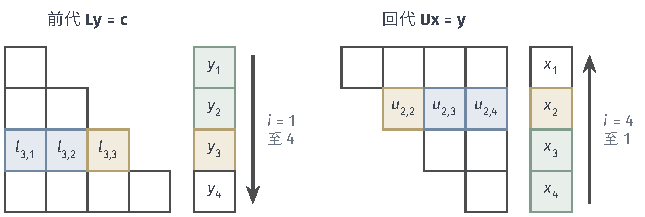
\includegraphics[width=109.1mm]{figures/01-basic-mathematics/03-vectors-matrices-and-multivariate-functions/tikz/c5-triangular-substitution-order/figure.pdf}
  \caption{前代与回代的计算顺序。左为四阶下三角方程，计算$y_3$时只用到第三行的蓝色元素与绿色的已算分量$y_1,y_2$；
  右为上三角方程，计算$x_2$时只用到$x_3,x_4$。黄色是当前用作除数的对角元与正在计算的分量，箭头是计算方向。}
  \label{fig:ls-triangular-substitution-order}
\end{figure}

\subsection{算法实现}
\label{sec:ls-lu-implementation}
输入是$\bm A$与$\bm b$，输出是$\bm x$。需要预先选定的规则是主元策略，本小节固定使用\term{部分选主元}：在当前列尚未处理的元素中选绝对值最大者作主元，绝对值相同时取行号最小者，使给定数据下的计算过程可以复算。算法由三个模块组成，下面依次给出：LU分解由$\bm A$算出$\bm P\bm A=\bm L\bm U$，前代求出$\bm y$，回代求出$\bm x$。下面逐个写出各模块的步骤，并在每一步用
\[
 \bm A=\begin{bmatrix}1&3&4\\2&2&4\\1&2&5\end{bmatrix},\qquad
 \bm b=\begin{bmatrix}2\\4\\4\end{bmatrix}
\]
演示该步的计算。

\subsubsection{LU分解}
输入$\bm A$，输出$\bm P$、$\bm L$、$\bm U$。消元逐列进行，用$k$记当前处理的列。计算中维护三个矩阵：工作矩阵$\bm W$逐步化为上三角形状，$\bm L$收集乘子，$\bm P$记录行交换。下面每一步之后都给出例中这三个矩阵的当前值。
\begin{enumerate}
 \item \textbf{初始化。}令$\bm W=\bm A$，$\bm L=\bm I_d$，$\bm P=\bm I_d$，$k=1$。

 例中
 \[
  \bm W=\begin{bmatrix}1&3&4\\2&2&4\\1&2&5\end{bmatrix},\quad
  \bm L=\begin{bmatrix}1&0&0\\0&1&0\\0&0&1\end{bmatrix},\quad
  \bm P=\begin{bmatrix}1&0&0\\0&1&0\\0&0&1\end{bmatrix}.
 \]

 \item \textbf{选主元并换行。}在第$k$列的第$k$至$d$行中找出主元所在的行
 \[
  r=\operatorname*{arg\,max}_{k\leq i\leq d}|w_{i,k}| ,
 \]
 交换$\bm W$的第$k,r$两行，并对$\bm P$作同样的行交换；$\bm L$前$k-1$列已经保存的乘子也交换这两行，使它们始终跟随所在的方程（理由见本节的算法分析）。若选出的主元为零，说明输入不满足非奇异的前提，停止并报告本算法不适用；$\bm A$非奇异时这种情况不会出现，理由见定理~\ref{thm:ls-lu-existence}。

 例中$k=1$，第一列为$(1,2,1)^\top$，绝对值最大的在第二行，$r=2$。交换$\bm W$与$\bm P$的第一、二行；$\bm L$的前$k-1=0$列中还没有乘子，不变：
 \[
  \bm W=\begin{bmatrix}2&2&4\\1&3&4\\1&2&5\end{bmatrix},\quad
  \bm L=\begin{bmatrix}1&0&0\\0&1&0\\0&0&1\end{bmatrix},\quad
  \bm P=\begin{bmatrix}0&1&0\\1&0&0\\0&0&1\end{bmatrix}.
 \]

 \item \textbf{计算乘子并更新尾块。}对每个$i>k$，把第$i$行减去第$k$行的$l_{i,k}$倍，以消去$w_{i,k}$。新的第$k$个元素是$w_{i,k}-l_{i,k}w_{k,k}$，令它为零，得乘子；同一次行操作也作用于该行其余的元素：
 \[
  l_{i,k}=\frac{w_{i,k}}{w_{k,k}},\qquad
  w_{i,j}\leftarrow w_{i,j}-l_{i,k}w_{k,j}\quad(j=k+1,\ldots,d),
 \]
 再令$w_{i,k}=0$，并把$l_{i,k}$存入$\bm L$的$(i,k)$位置。前$k-1$列在第$k$行和第$i$行上都已经是零，减去后仍为零，所以这一步只改变右下角的$(d-k)$阶尾块；$\bm P$不变。计算时使用的都是$\bm W$的当前值，而不是最初的$a_{i,j}$。

 例中$k=1$，乘子为$l_{2,1}=\tfrac12$、$l_{3,1}=\tfrac12$，两行的尾部更新为
 \[
  (3,4)-\tfrac12(2,4)=(2,2),\qquad(2,5)-\tfrac12(2,4)=(1,3),
 \]
 于是
 \[
  \bm W=\begin{bmatrix}2&2&4\\0&2&2\\0&1&3\end{bmatrix},\quad
  \bm L=\begin{bmatrix}1&0&0\\\tfrac12&1&0\\\tfrac12&0&1\end{bmatrix},\quad
  \bm P=\begin{bmatrix}0&1&0\\1&0&0\\0&0&1\end{bmatrix}.
 \]

 \item \textbf{判断是否结束。}若$k<d-1$，令$k\leftarrow k+1$，回到第2步处理下一列。若$k=d-1$，第$d$列下方已没有待消去的元素，所有列都已处理完毕，分解结束。

 例中$d=3$，$k=1<2$，于是令$k=2$回到第2步。第2步：第二列第二、三行的元素为$(2,1)^\top$，主元已在第二行，$r=2$，无需交换，三个矩阵都不变。第3步：乘子$l_{3,2}=\tfrac12$，第三行的尾部更新为$3-\tfrac12\cdot2=2$，得
 \[
  \bm W=\begin{bmatrix}2&2&4\\0&2&2\\0&0&2\end{bmatrix},\quad
  \bm L=\begin{bmatrix}1&0&0\\\tfrac12&1&0\\\tfrac12&\tfrac12&1\end{bmatrix},\quad
  \bm P=\begin{bmatrix}0&1&0\\1&0&0\\0&0&1\end{bmatrix}.
 \]
 这时$k=2=d-1$，分解结束，上式就是结束时三个矩阵的值。

 \item \textbf{取出因子。}第3步每次都把主元下方的元素置零，所以结束时$\bm W$的对角线下方全为零，它就是所求的上三角因子，取$\bm U=\bm W$；$\bm L$中已按位置填好全部乘子，就是单位下三角因子；$\bm P$记录了全部行交换。例中
 \[
  \bm U=\bm W=\begin{bmatrix}2&2&4\\0&2&2\\0&0&2\end{bmatrix},
 \]
 $\bm L$与$\bm P$取上面结束时的值。可以直接验证$\bm L\bm U$等于交换前两行后的$\bm A$，即$\bm P\bm A$。这项检查只涉及因子，与右端无关。
\end{enumerate}

上面的演示只在第一轮换行，已存乘子没有受到影响。下例在第二轮再次换行，用来检查第2步中“已存乘子随行交换”这条规则；例末的前代与回代按下面两小节进行。

\begin{example}[第二轮换行时交换已存乘子]
\label{ex:ls-lu-second-swap}
取
\[
 \bm A=\begin{bmatrix}0&2&1\\1&1&0\\2&0&1\end{bmatrix},\qquad
 \bm b=\begin{bmatrix}3\\2\\3\end{bmatrix}.
\]
第一轮，第一列中绝对值最大的是第三行的$2$，把第三行换到第一行，工作矩阵的行依次为$(2,0,1)$、$(1,1,0)$、$(0,2,1)$。乘子为$l_{2,1}=\tfrac12$、$l_{3,1}=0$，消元后两行变成$(0,1,-\tfrac12)$和$(0,2,1)$。

第二轮，第二列剩余元素为$1$与$2$，主元在第三行，交换后两行；同时把$\bm L$第一列中已存的乘子$\tfrac12$与$0$交换，使$l_{2,1}=0$、$l_{3,1}=\tfrac12$。再以$2$为主元，乘子$l_{3,2}=\tfrac12$，第三行变为$(0,1,-\tfrac12)-\tfrac12(0,2,1)=(0,0,-1)$。于是
\[
 \bm L=\begin{bmatrix}1&0&0\\0&1&0\\\tfrac12&\tfrac12&1\end{bmatrix},\qquad
 \bm U=\begin{bmatrix}2&0&1\\0&2&1\\0&0&-1\end{bmatrix},
\]
$\bm P\bm A$的三行依次是$\bm A$的第三、一、二行。逐行核对：$\bm L\bm U$的第三行为$\tfrac12(2,0,1)+\tfrac12(0,2,1)+(0,0,-1)=(1,1,0)$，正是$\bm A$的第二行；若忘记交换已存乘子，$\bm L$的第二行会是$(\tfrac12,1,0)$，乘出的第二行$(1,2,\tfrac32)$不再是$\bm P\bm A$的任何一行。

右端经两次交换为$\bm c=\bm P\bm b=(3,3,2)^\top$。前代依次得$y_1=3$、$y_2=3$、$y_3=2-\tfrac32-\tfrac32=-1$；回代得$x_3=(-1)/(-1)=1$、$x_2=(3-1)/2=1$、$x_1=(3-1)/2=1$。代回原方程，$\bm A\bm x=(3,2,3)^\top=\bm b$。
\end{example}

\subsubsection{前代}
输入$\bm P$、$\bm L$与$\bm b$，输出$\bm y$。
\begin{enumerate}
 \item \textbf{重排右端。}计算$\bm c=\bm P\bm b$，即对$\bm b$作与分解中相同的行交换。例中$\bm c=(4,2,4)^\top$。

 \item \textbf{逐个求出$y_i$。}根据式~\eqref{eq:ls-forward-substitution}，由于$l_{i,i}=1$，对$i=1,\ldots,d$依次得
 \[
  y_i=c_i-\sum_{j<i}l_{i,j}y_j ;
 \]
 求出$y_d$后结束。例中
 \[
  \begin{aligned}
  y_1&=c_1=4,\\
  y_2&=c_2-l_{2,1}y_1=2-\tfrac12\cdot4=0,\\
  y_3&=c_3-l_{3,1}y_1-l_{3,2}y_2=4-\tfrac12\cdot4-\tfrac12\cdot0=2 .
  \end{aligned}
 \]
\end{enumerate}

\subsubsection{回代}
输入$\bm U$与$\bm y$，输出$\bm x$。
\begin{enumerate}
 \item \textbf{逐个求出$x_i$。}根据式~\eqref{eq:ls-back-substitution}，对$i=d,\ldots,1$依次得
 \[
  x_i=\frac{y_i-\sum_{j>i}u_{i,j}x_j}{u_{i,i}} ;
 \]
 求出$x_1$后结束。例中
 \[
  \begin{aligned}
  x_3&=\frac{y_3}{u_{3,3}}=\frac22=1,\\
  x_2&=\frac{y_2-u_{2,3}x_3}{u_{2,2}}=\frac{0-2}{2}=-1,\\
  x_1&=\frac{y_1-u_{1,2}x_2-u_{1,3}x_3}{u_{1,1}}=\frac{4+2-4}{2}=1 .
  \end{aligned}
 \]

 \item \textbf{检验。}输出$\bm x$。精确算术下它就是$\bm x_\star$；浮点实现中还应报告缩放残差$\lVert\bm b-\bm A\bm x\rVert/(\lVert\bm A\rVert\lVert\bm x\rVert+\lVert\bm b\rVert)$，它的含义在第~\ref{sec:ls-numerical-stability}节解释。例中$\bm x=(1,-1,1)^\top$，代回得$\bm A\bm x=(2,4,4)^\top=\bm b$，残差为零。
\end{enumerate}
LU分解只依赖$\bm A$。换一个右端时，只需重做前代与回代。

\subsection{算法分析}
\paragraph{乘子与置换的拼合}
先说明LU分解第3步存入的乘子为什么恰好组成$\bm L$，以及第2步为什么要交换已存乘子。第$k$轮全部消元可以写成左乘一个矩阵。令$\bm\ell_k=(0,\ldots,0,l_{k+1,k},\ldots,l_{d,k})^\top$，前$k$个分量为零，则第$k$轮相当于左乘$\bm M_k=\bm I_d-\bm\ell_k\bm e_k^\top$：它把第$k$行的$l_{i,k}$倍从第$i$行减去。因为$\bm e_k^\top\bm\ell_k=0$，有
\[
 (\bm I_d-\bm\ell_k\bm e_k^\top)(\bm I_d+\bm\ell_k\bm e_k^\top)
 =\bm I_d-\bm\ell_k(\bm e_k^\top\bm\ell_k)\bm e_k^\top=\bm I_d,
\]
即$\bm M_k^{-1}=\bm I_d+\bm\ell_k\bm e_k^\top$。不交换行时，$\bm M_{d-1}\cdots\bm M_1\bm A=\bm U$，于是$\bm A=\bm M_1^{-1}\cdots\bm M_{d-1}^{-1}\bm U$。对$j<k$还有$\bm e_j^\top\bm\ell_k=0$，展开乘积时所有交叉项都消失，得到
\[
 \bm M_1^{-1}\cdots\bm M_{d-1}^{-1}=\bm I_d+\sum_{k=1}^{d-1}\bm\ell_k\bm e_k^\top=\bm L,
\]
所以乘子只需按位置填入$\bm L$，不需要另做矩阵乘法。

有行交换时，第$k$轮先左乘交换第$k,r$两行（$r\geq k$）的置换矩阵$\bm P_k$，再左乘$\bm M_k$。$\bm P_k$只交换下标不小于$k$的两个位置，对$j<k$有$\bm P_k\bm e_j=\bm e_j$，因此
\[
 \bm P_k\bm M_j=\bigl(\bm I_d-(\bm P_k\bm\ell_j)\bm e_j^\top\bigr)\bm P_k .
\]
这说明可以把$\bm P_k$移到此前的消元矩阵右侧，代价是把已经保存的乘子向量$\bm\ell_j$也交换第$k,r$两个分量。逐轮这样移动，全部置换合成$\bm P=\bm P_{d-1}\cdots\bm P_1$，便得到式~\eqref{eq:ls-palu}。这一推导也给出实现规则：后续交换两行时，$\bm L$中已经完成的前$k-1$列必须同时交换这两行，否则保存的乘子不再对应同一个方程。

\paragraph{正确性}
算法能否进行，取决于每一步是否有非零主元。部分选主元对任何非奇异矩阵都能进行；不选主元时则需要额外的条件，下面的定理给出这一条件，并说明分解在什么意义下唯一。

\begin{theorem}[LU分解的存在与唯一]
\label{thm:ls-lu-existence}
设$\bm A\in\mathbb R^{d\times d}$，记$\bm A_k$为其左上角$k$阶子矩阵。
\begin{enumerate}
 \item 若$\bm A$非奇异，则部分选主元消元的每一步都有非零主元，给出置换矩阵$\bm P$、元素满足$|l_{i,j}|\leq1$的单位下三角矩阵$\bm L$与非奇异上三角矩阵$\bm U$，使$\bm P\bm A=\bm L\bm U$。
 \item 不选主元时，$\bm A=\bm L\bm U$（$\bm L$单位下三角，$\bm U$非奇异上三角）存在，当且仅当$\det\bm A_k\neq0$对$k=1,\ldots,d$都成立；此时分解唯一。
\end{enumerate}
\end{theorem}
\begin{proof}
（1）第$k$步开始时$\bm W=\bm M\bm A$，其中$\bm M$是此前各次行交换与消元矩阵的乘积，可逆；$\bm W$的前$k-1$列已是对角元非零的上三角形状。若第$k$列从第$k$行起全为零，$\bm W$的前$k$列就都落在$\operatorname{span}\{\bm e_1,\ldots,\bm e_{k-1}\}$中而线性相关，$\bm A=\bm M^{-1}\bm W$随之奇异，矛盾。选出的主元绝对值最大，故$|l_{i,k}|\leq1$。由本小节开头的推导，全部置换移到右侧后得到$\bm P\bm A=\bm L\bm U$。

（2）若$\bm A=\bm L\bm U$，由三角形状，左上角$k$阶块满足$\bm A_k=\bm L_k\bm U_k$，故$\det\bm A_k=\prod_{i\leq k}u_{i,i}\neq0$。反之，设各$\det\bm A_k\neq0$，用归纳法说明不选主元时第$k$个主元非零：前$k-1$步只用了单位下三角的消元矩阵，$\bm W=\bm M\bm A$中$\bm M$单位下三角，于是$\bm W_k=\bm M_k\bm A_k$，$\det\bm W_k=\det\bm A_k\neq0$；而$\bm W_k$是上三角矩阵，前$k-1$个对角元非零，所以$w_{k,k}\neq0$。唯一性：若$\bm L_1\bm U_1=\bm L_2\bm U_2$，则$\bm L_2^{-1}\bm L_1=\bm U_2\bm U_1^{-1}$，左边单位下三角，右边上三角，只能都等于$\bm I_d$。
\end{proof}

定理的第一部分说明前代与回代给出的正是原方程的解：行交换只重排方程，不改变解。第二部分中的条件不能仅由$\bm A$非奇异推出，例如$\left[\begin{smallmatrix}0&1\\1&1\end{smallmatrix}\right]$可逆，第一个主元却为零。

\paragraph{主元增长与数值敏感度}
精确算术中任何非零主元都可以用，选主元是为有限精度服务的。主元很小时乘子很大，尾块更新$w_{i,j}-l_{i,k}w_{k,j}$会产生远大于原始元素的数，原始元素的信息在舍入中被淹没。衡量这种现象的是\term{增长因子}
\[
 \rho=\frac{\max_{i,j,k}|w^{(k)}_{i,j}|}{\max_{i,j}|a_{i,j}|},
\]
其中$w^{(k)}_{i,j}$是第$k$轮之后工作矩阵的元素。部分选主元使$|l_{i,k}|\leq1$，每轮元素的绝对值至多翻倍，所以$\rho\leq2^{d-1}$；这个上界可以达到，但在实际计算中极少出现，增长因子通常很小。LU的后向误差与$\rho$成正比，这一误差界及其解释见第~\ref{sec:ls-numerical-stability}节。

\paragraph{计算代价}
第$k$步更新$(d-k)^2$个元素，一次稠密分解约需$\tfrac23d^3$次浮点运算；此后每个新右端只需一次前代和一次回代，约$2d^2$次运算。因此求解$\bm A\bm X=\bm B$的$s$个右端总共约需$\tfrac23d^3+2sd^2$次运算，远少于对每个右端重新消元。稀疏矩阵消元时，原来为零的位置会产生非零元，称为\term{填充}（fill-in），其多少取决于消元顺序，估计代价时须一并考虑。

\section{Cholesky分解}
\label{sec:ls-cholesky}

对称正定矩阵是最常见的特殊结构，例如正规方程、二次型的Hessian矩阵和协方差矩阵。利用对称性，可以只构造一个三角因子，运算和存储都减少一半；正定性则保证构造过程中的每次开方和除法都能进行。

\subsection{主要思想}
设$\bm A\in\mathbb R^{d\times d}$实对称正定，$\bm b\in\mathbb R^d$，要求精确解$\bm x_\star$。核心思想是把LU中的两个三角因子取成互为转置的形式，即\term{Cholesky分解}（Cholesky decomposition）
\begin{equation}
 \bm A=\bm L\bm L^\top,
 \label{eq:matrix-analysis-cholesky}
\end{equation}
其中$\bm L$是对角元为正的下三角矩阵。这样只需构造一个因子$\bm L$，原方程$\bm L(\bm L^\top\bm x)=\bm b$就化为两个三角方程，用前代和回代各解一次。

\paragraph{逐元素等式}
构造$\bm L$的公式来自比较$\bm A$与$\bm L\bm L^\top$的元素。$\bm L\bm L^\top$的$(i,j)$元是$\bm L$的第$i$行与第$j$行的内积，因三角结构，$k>\min(i,j)$的项为零：
\[
 a_{i,j}=\sum_{k=1}^{\min(i,j)}l_{i,k}l_{j,k}.
\]
三阶时，下三角部分的六个等式依次是
\[
\begin{gathered}
 a_{1,1}=l_{1,1}^2,\quad a_{2,1}=l_{2,1}l_{1,1},\quad a_{3,1}=l_{3,1}l_{1,1},\\
 a_{2,2}=l_{2,1}^2+l_{2,2}^2,\quad a_{3,2}=l_{3,1}l_{2,1}+l_{3,2}l_{2,2},\\
 a_{3,3}=l_{3,1}^2+l_{3,2}^2+l_{3,3}^2 .
\end{gathered}
\]
按第一列、第二列、第三列的次序读这些等式，每个等式恰好只含一个新的未知元素，其余都已算出。

\paragraph{逐列递推}
一般地，在第$j$列先取$i=j$，把已完成列的贡献移到右侧，得$l_{j,j}^2=a_{j,j}-\sum_{k<j}l_{j,k}^2$；按正对角的约定取正根。再对同列下方的$i>j$，把$a_{i,j}=\sum_{k<j}l_{i,k}l_{j,k}+l_{i,j}l_{j,j}$中已知的部分移项，除以刚算出的$l_{j,j}$。合起来，对$j=1,\ldots,d$逐列计算
\begin{equation}
\begin{gathered}
 l_{j,j}=\sqrt{a_{j,j}-\sum_{k<j}l_{j,k}^2},\\
 l_{i,j}=\frac{a_{i,j}-\sum_{k<j}l_{i,k}l_{j,k}}{l_{j,j}}\quad(i>j),
\end{gathered}
\label{eq:ls-cholesky-columns}
\end{equation}
$j=1$时两个和式都是空和。计算的依赖方向是：先算本列对角元，再算其下全部元素，然后进入下一列；计算只读取$\bm A$的下三角部分。各列完成后，上述等式覆盖了下三角的全部位置，而$\bm A$与$\bm L\bm L^\top$都对称，上三角的等式自动成立，不需要另外计算。

\paragraph{开方量为什么为正}
式~\eqref{eq:ls-cholesky-columns}要求每个开方量为正，这正是正定性所保证的。设前$j-1$列已经算出，记左上角$j-1$阶块为$\bm B$，第$j$列在它上方的部分为$\bm c$，于是$\bm B=\bm L_{j-1}\bm L_{j-1}^\top$，其中$\bm L_{j-1}$是$\bm L$的左上角块。第$j$行已算出的前$j-1$个元素记为$\bm\ell$，由$a_{k,j}$（$k<j$）的等式得$\bm L_{j-1}\bm\ell=\bm c$，所以
\[
 \sum_{k<j}l_{j,k}^2=\lVert\bm\ell\rVert_2^2
 =\bm c^\top\bm L_{j-1}^{-\top}\bm L_{j-1}^{-1}\bm c
 =\bm c^\top\bm B^{-1}\bm c .
\]
开方量因而是$a_{j,j}-\bm c^\top\bm B^{-1}\bm c$，即左上角$j$阶块关于$\bm B$的Schur补。取前$j$个分量为$(-\bm B^{-1}\bm c,1)$、其余分量为零的向量$\bm w$，直接展开得
\[
 \bm w^\top\bm A\bm w
 =\bm c^\top\bm B^{-1}\bm c-2\bm c^\top\bm B^{-1}\bm c+a_{j,j}
 =a_{j,j}-\bm c^\top\bm B^{-1}\bm c,
\]
而$\bm w\neq\bm0$，正定性给出它严格为正。所以正定性不仅是输入的标签，它在每一列都以“开方量为正”的形式被使用。

\paragraph{两次三角求解}
最后由$\bm L(\bm L^\top\bm x)=\bm b$，先用前代~\eqref{eq:ls-forward-substitution}求解$\bm L\bm y=\bm b$，再用回代~\eqref{eq:ls-back-substitution}求解$\bm L^\top\bm x=\bm y$，即
\[
 y_i=\frac{b_i-\sum_{k<i}l_{i,k}y_k}{l_{i,i}},\qquad
 x_i=\frac{y_i-\sum_{k>i}l_{k,i}x_k}{l_{i,i}} .
\]
与LU不同，这里$l_{i,i}$一般不等于$1$，除法要保留；$\bm L^\top$的上三角元素$(\bm L^\top)_{i,k}=l_{k,i}$直接从$\bm L$读出，同一个因子分别按正序和逆序读取，无需显式计算$\bm A^{-1}$。

\subsection{算法实现}
\paragraph{逐列分解}
输入实对称正定的$\bm A$和$\bm b$，把$\bm L$初始化为零矩阵。对$j=1,\ldots,d$，先累计开方量$\delta_j=a_{j,j}-\sum_{k<j}l_{j,k}^2$，检查$\delta_j>0$后令$l_{j,j}=\sqrt{\delta_j}$；再对$i=j+1,\ldots,d$累计列内乘积和，按式~\eqref{eq:ls-cholesky-columns}计算$l_{i,j}$。

若某个$\delta_j\leq0$，就停止并报告：要么输入不满足正定条件，要么矩阵接近奇异，舍入误差已使当前计算不可靠。这时不能擅自取绝对值继续，也不能把小量截为零后当作Cholesky分解；对称不定问题改用第~\ref{sec:ls-ldlt}节的分块LDL分解，半正定或秩亏问题按求解目标改用第~\ref{sec:ls-svd-solve}节的SVD求解或第~\ref{chap:solution-error-regularization}章的正则化。

\paragraph{两次三角求解}
分解完成后，前代求解$\bm L\bm y=\bm b$，回代求解$\bm L^\top\bm x=\bm y$，输出$\bm x$。实际程序只保存下三角因子；多个右端复用同一因子。

\begin{example}[Cholesky分解的三步计算]
\label{ex:ls-cholesky-three-steps}
取
\[
 \bm A=\begin{bmatrix}4&2&2\\2&5&3\\2&3&6\end{bmatrix},\qquad
 \bm b=\begin{bmatrix}8\\10\\11\end{bmatrix}.
\]
这个矩阵对称正定，可以用Cholesky分解。逐列计算：第一列$l_{1,1}=\sqrt4=2$，$l_{2,1}=l_{3,1}=2/2=1$；第二列先扣除第一列的贡献再开方，$l_{2,2}=\sqrt{5-1}=2$，$l_{3,2}=(3-1\cdot1)/2=1$；最后$l_{3,3}=\sqrt{6-1-1}=2$，即
\[
 \bm L=\begin{bmatrix}2&0&0\\1&2&0\\1&1&2\end{bmatrix}.
\]
只有一个因子，前代用$\bm L$，回代用它的转置。前代解$\bm L\bm y=\bm b$，得$y_1=8/2=4$，$y_2=(10-4)/2=3$，$y_3=(11-4-3)/2=2$；回代解$\bm L^\top\bm x=\bm y$，得$x_3=2/2=1$，$x_2=(3-1)/2=1$，$x_1=(4-1-1)/2=1$。所以$\bm x=(1,1,1)^\top$，代回可验$\bm A\bm x=\bm b$。
\end{example}

上例各元素都为正。下例含负的非对角元，用来检查递推中各项的符号，并分别核验分解残差和求解残差。

\begin{example}[含负元素的Cholesky分解与核验]
\label{ex:ls-cholesky-signed}
取
\[
 \bm A=\begin{bmatrix}4&12&-16\\12&37&-43\\-16&-43&98\end{bmatrix},\qquad
 \bm b=\begin{bmatrix}0\\6\\39\end{bmatrix}.
\]
第一列：$l_{1,1}=\sqrt4=2$，$l_{2,1}=12/2=6$，$l_{3,1}=-16/2=-8$。第二列：开方量$37-6^2=1$，所以$l_{2,2}=1$；$l_{3,2}=(-43-(-8)\cdot6)/1=5$。第三列：开方量$98-(-8)^2-5^2=9$，所以$l_{3,3}=3$。于是
\[
 \bm L=\begin{bmatrix}2&0&0\\6&1&0\\-8&5&3\end{bmatrix},
\]
逐项相乘可验$\bm L\bm L^\top=\bm A$，例如$(3,2)$元为$(-8)\cdot6+5\cdot1=-43$。

前代依次得$y_1=0/2=0$，$y_2=(6-6\cdot0)/1=6$，$y_3=(39-(-8)\cdot0-5\cdot6)/3=3$；回代解$\bm L^\top\bm x=\bm y$，得$x_3=3/3=1$，$x_2=(6-5\cdot1)/1=1$，$x_1=(0-6\cdot1-(-8)\cdot1)/2=1$。最后用原始的$\bm A$和$\bm b$重算$\bm A\bm x-\bm b$，本例为零。分解残差$\bm A-\bm L\bm L^\top$检查因子，求解残差$\bm b-\bm A\bm x$检查两次三角求解，二者要分别核验。
\end{example}

\subsection{算法分析}
\paragraph{正确性}
逐列构造能否进行，取决于每次开方的数是否为正。主要思想中已经看到正定性保证了这一点；下面的定理进一步说明正定性也是分解存在的必要条件。

\begin{theorem}[Cholesky分解的存在与唯一]
\label{thm:ls-cholesky-existence}
设$\bm A\in\mathbb R^{d\times d}$对称。存在对角元为正的下三角矩阵$\bm L$使$\bm A=\bm L\bm L^\top$，当且仅当$\bm A\succ0$；此时$\bm L$唯一，并由式~\eqref{eq:ls-cholesky-columns}给出。
\end{theorem}
\begin{proof}
必要性：$\bm L$的对角元为正，故可逆；对非零$\bm v$有$\bm v^\top\bm A\bm v=\lVert\bm L^\top\bm v\rVert_2^2>0$。充分性对阶数归纳。把$\bm A$按首行首列分块为$\left[\begin{smallmatrix}a_{1,1}&\bm a^\top\\\bm a&\bm A_{22}\end{smallmatrix}\right]$，正定性给出$a_{1,1}=\bm e_1^\top\bm A\bm e_1>0$，所以$l_{1,1}=\sqrt{a_{1,1}}$有定义，第一列其余元素为$\bm a/l_{1,1}$。对$\bm v=(v_1,\bm w^\top)^\top$关于首变量配方，
\[
\begin{aligned}
 \bm v^\top\bm A\bm v
 &=a_{1,1}\Bigl(v_1+\frac{\bm a^\top\bm w}{a_{1,1}}\Bigr)^2\\
 &\quad+\bm w^\top\Bigl(\bm A_{22}-\frac{\bm a\bm a^\top}{a_{1,1}}\Bigr)\bm w .
\end{aligned}
\]
对任意非零$\bm w$取$v_1=-\bm a^\top\bm w/a_{1,1}$，左边为正，故剩余矩阵$\bm A_{22}-\bm a\bm a^\top/a_{1,1}$仍正定；后面各列的计算正是对它重复同样的步骤，由归纳假设每一步开方的数都为正。唯一性：对角元取正后，式~\eqref{eq:ls-cholesky-columns}逐个唯一地确定每个元素。
\end{proof}

由$\bm A=\bm L\bm L^\top$，算出的$\bm x$满足$\bm A\bm x=\bm L(\bm L^\top\bm x)=\bm L\bm y=\bm b$。

\paragraph{数值敏感度}
$a_{j,j}=\sum_{k\leq j}l_{j,k}^2$给出$|l_{j,k}|\leq\sqrt{a_{j,j}}$，因子的元素不会增长，因此分解不选主元也是后向稳定的（第~\ref{sec:ls-numerical-stability}节）；解的误差仍由$\bm A$的条件数决定（第~\ref{sec:ls-matrix-condition-number}节）。还要区分数学上的正定与有限精度下的可计算性：$\bm A$正定但最小特征值相对于$\lVert\bm A\rVert_2$极小时，开方量本身很小，舍入误差可能使它算成零或负数，算法在一个本应正定的矩阵上报告失败。这种失败提示问题接近奇异，处理办法属于第~\ref{chap:solution-error-regularization}章。

\paragraph{计算代价}
稠密分解约需$\tfrac13d^3$次运算，是LU的一半，存储也只需一个三角因子；每个右端的两次三角求解约需$2d^2$次运算。

\section{分块LDL分解}
\label{sec:ls-ldlt}

对称但不定的矩阵也很常见，例如带约束的二次问题给出的鞍点系统。这时Cholesky分解的开方量可能为负，而直接用LU又浪费了对称性。分块LDL分解不开方，并在必要时用二阶主元块，使对称结构和非奇异方程的可解性同时得到保留。

\subsection{主要思想}
设$\bm A\in\mathbb R^{d\times d}$实对称非奇异，但不一定正定，$\bm b\in\mathbb R^d$，要求唯一精确解$\bm x_\star$。目标是构造\term{分块LDL分解}
\begin{equation}
 \bm P\bm A\bm P^\top=\bm L\bm D\bm L^\top,
 \label{eq:ls-ldlt}
\end{equation}
其中$\bm P$是置换矩阵，$\bm L$是单位下三角矩阵，$\bm D$由可逆的一阶和二阶对称块组成。对称置换同时交换行与列，矩阵保持对称。

\paragraph{标量主元的递推}
先看无需交换、每个主元都是非零标量的情形。设$\bm A=\bm L\bm D\bm L^\top$，$\bm D=\operatorname{diag}(d_1,\ldots,d_d)$，比较$(i,j)$元（$i\geq j$）得$a_{i,j}=\sum_{k\leq j}l_{i,k}d_kl_{j,k}$。与Cholesky的推导相同，逐列移项得到
\[
 d_j=a_{j,j}-\sum_{k<j}l_{j,k}^2d_k,\qquad
 l_{i,j}=\frac{a_{i,j}-\sum_{k<j}l_{i,k}d_kl_{j,k}}{d_j}\quad(i>j).
\]
这里不对$d_j$开方，所以$d_j$可以为负，主元的正负号保留在$\bm D$中；但仍要除以$d_j$，零主元会使递推中断。

\paragraph{为什么需要二阶块}
零主元并不意味着矩阵奇异。例如$\left[\begin{smallmatrix}0&1\\1&0\end{smallmatrix}\right]$可逆，但两个对角元都是零。对称置换只把对角元换到别的对角位置，所以无论怎样对称交换，第一个标量主元都是零；若据此判定矩阵奇异就会出错。把这两行两列合成一个可逆的二阶块作主元，才保留方程的可解性。

\paragraph{一步块消元}
设交换后当前剩余矩阵写成
\[
 \begin{bmatrix}\bm E&\bm C^\top\\\bm C&\bm F\end{bmatrix},
\]
其中$\bm E$是选出的一阶或二阶可逆对称块。要找乘子块$\bm M$与新的剩余矩阵$\bm S$，使
\[
 \begin{bmatrix}\bm E&\bm C^\top\\\bm C&\bm F\end{bmatrix}
 =\begin{bmatrix}\bm I&\bm0\\\bm M&\bm I\end{bmatrix}
 \begin{bmatrix}\bm E&\bm0\\\bm0&\bm S\end{bmatrix}
 \begin{bmatrix}\bm I&\bm M^\top\\\bm0&\bm I\end{bmatrix}.
\]
右侧乘开后左下块为$\bm M\bm E$，右下块为$\bm M\bm E\bm M^\top+\bm S$。令左下块等于$\bm C$，得$\bm M\bm E=\bm C$，即$\bm M=\bm C\bm E^{-1}$；令右下块等于$\bm F$，并用$\bm E$对称化简$\bm M\bm E\bm M^\top=\bm C\bm E^{-1}\bm C^\top=\bm M\bm C^\top$，得
\[
 \bm S=\bm F-\bm M\bm C^\top=\bm F-\bm C\bm E^{-1}\bm C^\top .
\]
实际计算时通过求解一阶或二阶方程$\bm M\bm E=\bm C$形成$\bm M$，不显式求逆。

\paragraph{分解与求解}
对$\bm S$重复同样的步骤，并把每一轮的对称置换累积起来，就得到式~\eqref{eq:ls-ldlt}。由它，$\bm A\bm x=\bm b$等价于$\bm L\bm D\bm L^\top(\bm P\bm x)=\bm P\bm b$，求解依次为$\bm L\bm y=\bm P\bm b$、$\bm D\bm z=\bm y$、$\bm L^\top\bm w=\bm z$和$\bm x=\bm P^\top\bm w$。中间一步按$\bm D$的对角块求解，而不是逐元素相除。

\subsection{算法实现}
需要预先选定的规则是选块策略。为使给定数据下的计算可以复算，这里采用一个精确算术下可执行的代数规则。设当前剩余矩阵的首个对角元为$w_{k,k}$：若$w_{k,k}\neq0$，取它作一阶块；若$w_{k,k}=0$，在第$k$列下方找绝对值最大的非零元素$w_{p,k}$（绝对值相同时取行号最小者），把第$p$行与第$p$列对称地交换到第$k+1$个位置，取二阶块
\[
 \bm E=\begin{bmatrix}0&w_{p,k}\\w_{p,k}&w_{p,p}\end{bmatrix},
\]
它的行列式为$-w_{p,k}^2\neq0$，所以可逆；若第$k$列下方也全为零，报告非奇异分支失败。这一规则只保证构造能够进行，并不保证数值稳定。

\paragraph{选块与对称交换}
初始化$\bm W=\bm A$、$\bm L=\bm I_d$、$\bm P=\bm I_d$，$\bm D$为空。每一轮按选块规则确定一阶或二阶块，需要交换时同时交换$\bm W$的相应行与列，对$\bm P$作同样的行交换，$\bm L$中已经算出的乘子也交换相应两行。交换后把当前剩余矩阵写成主要思想中的分块形式，$\bm E$为选出的主元块。

\paragraph{块消元}
逐行求解一阶或二阶方程$\bm M\bm E=\bm C$得到乘子块$\bm M$。把$\bm M$写入$\bm L$中主元块下方的位置，把$\bm E$放入$\bm D$的下一个对角块，再把剩余矩阵更新为
\[
 \bm F-\bm M\bm C^\top .
\]
它仍是对称矩阵，只需计算下三角部分。下一轮的起点前移的步长等于本轮主元块的阶数；对更小的剩余矩阵重复选块与消元，直到剩余矩阵为空。

\paragraph{三段求解}
先把右端重排为$\bm c=\bm P\bm b$，用前代求解$\bm L\bm y=\bm c$。接着按$\bm D$的对角块逐个求解$\bm D\bm z=\bm y$：一阶块直接作标量除法；对二阶块$\left[\begin{smallmatrix}e_{1,1}&e_{1,2}\\e_{1,2}&e_{2,2}\end{smallmatrix}\right]$，把它对应的两个分量记为$(y_1,y_2)$与$(z_1,z_2)$，由二阶逆矩阵公式得
\[
\begin{gathered}
 z_1=\frac{e_{2,2}y_1-e_{1,2}y_2}{e_{1,1}e_{2,2}-e_{1,2}^2},\\
 z_2=\frac{e_{1,1}y_2-e_{1,2}y_1}{e_{1,1}e_{2,2}-e_{1,2}^2},
\end{gathered}
\]
分母因所选块可逆而非零。最后用回代求解$\bm L^\top\bm w=\bm z$，此时$\bm w=\bm P\bm x$，再按$\bm x=\bm P^\top\bm w$恢复未知量的原次序，得到所求的$\bm x$。

\begin{example}[需要二阶块的LDL分解]
\label{ex:ls-ldlt-two-by-two}
取
\[
 \bm A=\begin{bmatrix}0&2&1\\2&0&1\\1&1&0\end{bmatrix},\qquad
 \bm b=\begin{bmatrix}3\\3\\2\end{bmatrix}.
\]
这个矩阵的对角元全为零，不能取一阶主元，Cholesky分解也无从开始。第一列下方绝对值最大的元素是$a_{2,1}=2$，它已在第二个位置，所以$\bm P=\bm I_3$，取二阶块$\bm E=\left[\begin{smallmatrix}0&2\\2&0\end{smallmatrix}\right]$，其余部分为$\bm C=(1,1)$、$\bm F=0$。由$\bm M\bm E=\bm C$得$\bm M=(\tfrac12,\tfrac12)$，剩余矩阵为$0-\bm M\bm C^\top=-1$，于是$\bm D=\operatorname{diag}(\bm E,-1)$，$\bm L$的第三行为$(\tfrac12,\tfrac12,1)$。

求解分三段。前代得$\bm y=(3,3,2-\tfrac32-\tfrac32)^\top=(3,3,-1)^\top$；再按$\bm D$的块结构求解，二阶块给出$z_1=z_2=(0-6)/(-4)=\tfrac32$，一阶块给出$z_3=1$；最后回代，得$w_3=1$，$w_2=w_1=\tfrac32-\tfrac12=1$。因此$\bm x=(1,1,1)^\top$，代回可验$\bm A\bm x=\bm b$。
\end{example}

上例三个对角元都是零。下例的第三个对角元非零，二阶块之后的剩余矩阵为负数，用来同时观察二阶块的求解和负主元的保留。

\begin{example}[二阶块后接负主元]
\label{ex:ls-ldlt-negative-pivot}
取
\[
 \bm A=\begin{bmatrix}0&1&1\\1&0&2\\1&2&3\end{bmatrix},\qquad
 \bm b=\begin{bmatrix}2\\3\\6\end{bmatrix}.
\]
首个对角元为零，第一列下方绝对值最大的元素是$a_{2,1}=1$（与$a_{3,1}$相同，取行号较小者），无需交换，取$\bm E=\left[\begin{smallmatrix}0&1\\1&0\end{smallmatrix}\right]$，$\bm C=(1,2)$，$\bm F=3$。设$\bm M=(m_1,m_2)$，则$\bm M\bm E=(m_2,m_1)=(1,2)$，得$\bm M=(2,1)$；剩余矩阵为$3-(2,1)(1,2)^\top=-1$。因此
\[
 \bm L=\begin{bmatrix}1&0&0\\0&1&0\\2&1&1\end{bmatrix},\qquad
 \bm D=\begin{bmatrix}0&1&0\\1&0&0\\0&0&-1\end{bmatrix}.
\]
前代得$\bm y=(2,3,6-2\cdot2-1\cdot3)^\top=(2,3,-1)^\top$。二阶块方程$z_2=2$、$z_1=3$，一阶块给出$z_3=(-1)/(-1)=1$，即$\bm z=(3,2,1)^\top$。回代得$w_3=1$，$w_2=2-1\cdot1=1$，$w_1=3-2\cdot1=1$；本例无需置换，所以$\bm x=\bm w=(1,1,1)^\top$。逐项可验$\bm L\bm D\bm L^\top=\bm A$与$\bm A\bm x=\bm b$。最后出现的两个$-1$含义不同：二阶块的行列式$\det\bm E=-1$非零，说明所选块可逆、消元可以进行；末尾主元$-1$非零，则与$\bm E$一起保证整个矩阵非奇异，$\det\bm A=\det\bm E\cdot(-1)=1$。
\end{example}

\subsection{算法分析}
\paragraph{正确性}
主要思想中的一步块消元恒等式可以乘开验证，只用到$\bm M\bm E=\bm C$和$\bm E^\top=\bm E$。两侧单位块三角因子的行列式为$1$，对称置换$\bm P\bm W\bm P^\top$也不改变行列式，所以每一轮的剩余矩阵都与$\bm A$一样非奇异。选块规则因此总能进行：若当前首个对角元为零且第$k$列下方也全为零，则由对称性剩余矩阵的首行首列全为零，它将是奇异的，矛盾。逐轮累积对称置换与乘子即得式~\eqref{eq:ls-ldlt}，前代、块对角求解、回代与还原次序因而给出原方程的解。$\bm D$中的负主元或不定二阶块只说明$\bm A$有使二次型为负的方向，并不妨碍可逆求解。

\paragraph{数值敏感度}
要区分两类规则：上面的选块规则保证代数构造可以进行，稳定的主元策略则要控制数值误差。存在可逆主元并不等于稳定：主元块相对很小时乘子很大，剩余矩阵的元素随之增长，与LU中的主元增长是同一现象。实用的选块策略要控制这种增长，Bunch--Kaufman策略就是一例，它按当前对角元与所在列最大非对角元的相对大小，决定取一阶块还是二阶块。

\paragraph{计算代价}
稠密计算约需$\tfrac13d^3$次运算，存储约$\tfrac12d^2$个元素，利用对称性比直接用LU减少一半。

\section{低秩更新下的求解}
\label{sec:ls-woodbury}

实际计算中常常要连续求解一系列只相差少量修改的方程，例如新增或删除一个约束、调整一个参数后重新求解。若每次修改的秩很小，就不必重新分解整个矩阵，而可以复用旧矩阵的分解，只多解一个低阶系统。这一节省依赖两个前提：旧分解已经存在，并且修改的秩远小于矩阵阶数。

\subsection{主要思想}
设新的系数矩阵具有已知结构
\[
 \bm A=\bm A_0+\bm U\bm C\bm V^\top,
\]
其中$\bm A_0\in\mathbb R^{d\times d}$非奇异，$\bm U,\bm V\in\mathbb R^{d\times k}$，$\bm C\in\mathbb R^{k\times k}$，$k\ll d$，且$\bm A$非奇异；要求$\bm A\bm x=\bm b$的精确解。更新表示是输入矩阵的结构信息，$\bm A_0$已有的分解只在内部复用。$\bm C$可以吸收修改项中的系数；取$\bm C=\bm I_k$就是常见的$\bm A_0+\bm U\bm V^\top$。

\paragraph{辅助变量}
修改项$\bm U\bm C\bm V^\top\bm x$只通过$k$维量$\bm C\bm V^\top\bm x$影响方程。令$\bm z=\bm C\bm V^\top\bm x$，原方程写成$\bm A_0\bm x=\bm b-\bm U\bm z$。用$\bm A_0$的因子求解$\bm A_0\bm u=\bm b$与$\bm A_0\bm Z=\bm U$，就得到
\[
 \bm x=\bm u-\bm Z\bm z .
\]
两边左乘$\bm C\bm V^\top$，由$\bm z$的定义得$\bm z=\bm C\bm V^\top\bm u-\bm C\bm V^\top\bm Z\bm z$，移项便是$k$阶方程
\[
 \bm K\bm z=\bm h,\qquad
 \bm K=\bm I_k+\bm C\bm V^\top\bm Z,\quad
 \bm h=\bm C\bm V^\top\bm u .
\]
所以完整的计算只需要旧因子上的$k+1$个右端求解，以及一个$k$阶辅助方程的求解；解出$\bm z$后代回$\bm x=\bm u-\bm Z\bm z$。

\paragraph{秩一修改}
最常见的是秩一修改$\bm A=\bm A_0+\bm p\bm q^\top$，即$k=1$、$\bm U=\bm p$、$\bm V=\bm q$、$\bm C=1$。这时$\bm Z$是一个向量，记$\bm A_0\bm w=\bm p$，辅助方程退化为标量除法：
\[
 z=\frac{\bm q^\top\bm u}{1+\bm q^\top\bm w},\qquad \bm x=\bm u-z\bm w .
\]
分母为零表示更新后的矩阵奇异（定理~\ref{thm:ls-sherman-morrison}）；分母很小则提示结果可能对舍入很敏感，低阶运算并不自动意味着稳定。

\subsection{算法实现}
\paragraph{用旧因子求解}
先取得$\bm A_0$的分解。它通常已经存在，可以直接复用；尚无分解时先按$\bm A_0$的结构调用前面的方法求得。下面关于节省计算的比较，以分解已经存在为前提。用这组因子求解$\bm A_0\bm u=\bm b$，得到未作更新时的解$\bm u$；再对$\bm U$的$k$列复用同一组因子，求解$\bm A_0\bm Z=\bm U$，得到$\bm Z\in\mathbb R^{d\times k}$，它记录修改方向经$\bm A_0^{-1}$作用后的结果。

\paragraph{形成小系统}
形成$k$阶矩阵$\bm K=\bm I_k+\bm C\bm V^\top\bm Z$与$k$维向量$\bm h=\bm C\bm V^\top\bm u$。计算时先算$\bm V^\top\bm Z$与$\bm V^\top\bm u$，再左乘$\bm C$，全程不形成新的$d$阶矩阵。

\paragraph{求解小系统并修正}
调用已有的直接法求解$\bm K\bm z=\bm h$；$\bm K$奇异时停止，因为更新后的矩阵也奇异。再计算$\bm x=\bm u-\bm Z\bm z$，得到新方程的解。每次修正之后都应在更新后的矩阵下重算原残差$\bm b-\bm A\bm x$，而不是只检查辅助方程。

\begin{example}[秩一更新的计算]
\label{ex:ls-woodbury-rank-one}
把二阶贯穿例看成一个易解矩阵加上秩一修改：$\bm A=\left[\begin{smallmatrix}4&1\\1&3\end{smallmatrix}\right]$等于$\bm A_0=\operatorname{diag}(3,2)$加上$\bm U\bm C\bm V^\top$，其中$\bm U=\bm V=(1,1)^\top$，$\bm C=1$；右端$\bm b=(1,2)^\top$。$\bm A_0$是对角矩阵，用它求解只需逐个相除，得$\bm u=(\tfrac13,1)^\top$，$\bm Z=(\tfrac13,\tfrac12)^\top$。

修改的秩为一，小系统只是一个标量方程：$\bm K=1+\tfrac13+\tfrac12=\tfrac{11}6$，$\bm h=\tfrac13+1=\tfrac43$，于是$\bm z=\tfrac43\cdot\tfrac6{11}=\tfrac8{11}$。修正后
\[
 \bm x=\begin{bmatrix}\tfrac13\\1\end{bmatrix}-\frac8{11}\begin{bmatrix}\tfrac13\\\tfrac12\end{bmatrix}
 =\begin{bmatrix}\tfrac1{11}\\\tfrac7{11}\end{bmatrix},
\]
代回可验$\bm A\bm x=(\tfrac4{11}+\tfrac7{11},\tfrac1{11}+\tfrac{21}{11})^\top=(1,2)^\top=\bm b$，全程没有分解$\bm A$本身。
\end{example}

上例的修改是对称的。下例取$\bm U\neq\bm V$，修改后的矩阵不再对称，但计算步骤不变。

\begin{example}[非对称的秩一更新]
\label{ex:ls-woodbury-nonsymmetric}
取$\bm A_0=\operatorname{diag}(2,3)$，$\bm U=(1,1)^\top$，$\bm V=(1,0)^\top$，$\bm C=1$，$\bm b=(4,5)^\top$，更新后的矩阵为$\bm A=\left[\begin{smallmatrix}3&0\\1&3\end{smallmatrix}\right]$。旧因子给出$\bm u=(2,\tfrac53)^\top$与$\bm Z=(\tfrac12,\tfrac13)^\top$。小系统为$\bm K=1+\bm V^\top\bm Z=\tfrac32$、$\bm h=\bm V^\top\bm u=2$，所以$z=\tfrac43$，修正得
\[
 \bm x=\begin{bmatrix}2\\\tfrac53\end{bmatrix}-\frac43\begin{bmatrix}\tfrac12\\\tfrac13\end{bmatrix}
 =\begin{bmatrix}\tfrac43\\\tfrac{11}9\end{bmatrix}.
\]
用更新后的矩阵重算：$3\cdot\tfrac43=4$，$\tfrac43+3\cdot\tfrac{11}9=5$，原残差为零。若连续作多次更新，辅助系统可能逐渐病态，误差也会累积，这时应与重新分解的代价比较，而不无限复用旧因子。
\end{example}

\subsection{算法分析}
\paragraph{正确性}
主要思想已经说明原方程的解满足$\bm x=\bm u-\bm Z\bm z$与$\bm K\bm z=\bm h$。反过来，若$\bm K\bm z=\bm h$且$\bm x=\bm u-\bm Z\bm z$，则$\bm C\bm V^\top\bm x=\bm h-(\bm K-\bm I_k)\bm z=\bm z$，从而$\bm A\bm x=\bm A_0\bm x+\bm U\bm z=\bm b$。所以小系统与原方程等价。把这一等价关系对任意右端写成矩阵形式，就得到下面的可逆性判据与逆矩阵公式。

\begin{theorem}[Woodbury恒等式]
\label{thm:ls-woodbury}
设$\bm A_0\in\mathbb R^{d\times d}$可逆，$\bm U,\bm V\in\mathbb R^{d\times k}$，$\bm C\in\mathbb R^{k\times k}$，记$\bm K=\bm I_k+\bm C\bm V^\top\bm A_0^{-1}\bm U$。则
\[
 \det(\bm A_0+\bm U\bm C\bm V^\top)=\det\bm A_0\det\bm K,
\]
因而$\bm A_0+\bm U\bm C\bm V^\top$可逆当且仅当$\bm K$可逆。若$\bm C$也可逆且$\bm K$可逆，则成立\term{Woodbury恒等式}（Woodbury identity）
\begin{equation}
\begin{aligned}
 &(\bm A_0+\bm U\bm C\bm V^\top)^{-1}\\
 &=\bm A_0^{-1}-\bm A_0^{-1}\bm U
 (\bm C^{-1}+\bm V^\top\bm A_0^{-1}\bm U)^{-1}
 \bm V^\top\bm A_0^{-1}.
\end{aligned}
\label{eq:matrix-analysis-woodbury}
\end{equation}
\end{theorem}
\begin{proof}
记$\bm Z=\bm A_0^{-1}\bm U$，则$\bm A_0+\bm U\bm C\bm V^\top=\bm A_0(\bm I_d+\bm Z\bm C\bm V^\top)$。分块矩阵$\bm T=\left[\begin{smallmatrix}\bm I_d&-\bm Z\\\bm C\bm V^\top&\bm I_k\end{smallmatrix}\right]$有两种分块三角分解，直接相乘即可验证：
\[
 \begin{aligned}
 \bm T&=\begin{bmatrix}\bm I_d&\bm0\\\bm C\bm V^\top&\bm I_k\end{bmatrix}
 \begin{bmatrix}\bm I_d&-\bm Z\\\bm0&\bm I_k+\bm C\bm V^\top\bm Z\end{bmatrix}\\
 &=\begin{bmatrix}\bm I_d+\bm Z\bm C\bm V^\top&-\bm Z\\\bm0&\bm I_k\end{bmatrix}
 \begin{bmatrix}\bm I_d&\bm0\\\bm C\bm V^\top&\bm I_k\end{bmatrix}.
 \end{aligned}
\]
分块三角矩阵的行列式等于对角块行列式之积，两种分解分别给出$\det\bm T=\det(\bm I_k+\bm C\bm V^\top\bm Z)$与$\det\bm T=\det(\bm I_d+\bm Z\bm C\bm V^\top)$，所以$\det(\bm I_d+\bm Z\bm C\bm V^\top)=\det\bm K$，第一个结论成立。$\bm C$可逆时$\bm K=\bm C(\bm C^{-1}+\bm V^\top\bm A_0^{-1}\bm U)$，括号内的矩阵随$\bm K$可逆。由上面的等价关系，对任意$\bm b$，新方程的解为$\bm x=\bm u-\bm Z\bm K^{-1}\bm C\bm V^\top\bm u$，其中$\bm u=\bm A_0^{-1}\bm b$；代入$\bm K^{-1}\bm C=(\bm C^{-1}+\bm V^\top\bm A_0^{-1}\bm U)^{-1}$，并因$\bm b$任意而去掉右端，即得式~\eqref{eq:matrix-analysis-woodbury}。
\end{proof}

判据部分允许$\bm C$奇异，这正是算法只使用$\bm K$、不使用$\bm C^{-1}$的原因。秩一修改时，定理化为一个只含标量分母的公式。

\begin{theorem}[Sherman--Morrison公式]
\label{thm:ls-sherman-morrison}
设$\bm A_0\in\mathbb R^{d\times d}$可逆，$\bm p,\bm q\in\mathbb R^d$。则$\bm A_0+\bm p\bm q^\top$可逆当且仅当$1+\bm q^\top\bm A_0^{-1}\bm p\neq0$，此时
\[
 (\bm A_0+\bm p\bm q^\top)^{-1}
 =\bm A_0^{-1}-\frac{\bm A_0^{-1}\bm p\bm q^\top\bm A_0^{-1}}{1+\bm q^\top\bm A_0^{-1}\bm p}.
\]
\end{theorem}
\begin{proof}
在定理~\ref{thm:ls-woodbury}中取$k=1$、$\bm U=\bm p$、$\bm V=\bm q$、$\bm C=1$，则$\bm K=1+\bm q^\top\bm A_0^{-1}\bm p$是标量，$(\bm C^{-1}+\bm V^\top\bm A_0^{-1}\bm U)^{-1}=1/\bm K$，代入式~\eqref{eq:matrix-analysis-woodbury}即得。
\end{proof}

\paragraph{数值敏感度}
代数恒等式并不自动保证数值稳定。$\bm K$接近奇异时，小系统的求解会放大误差；$\bm A_0$的求解本身敏感时，$\bm u$与$\bm Z$的误差即使在$\bm A$良态时也会进入结果；$\bm u$与$\bm Z\bm z$大小相近时，相减还会发生相消。

\paragraph{计算代价}
已有因子时，$k+1$个右端的三角求解约需$O(kd^2)$次运算，形成$\bm V^\top\bm Z$约需$O(k^2d)$，求解小系统约需$O(k^3)$，合计$O(kd^2+k^2d+k^3)$；优势来自$k$远小于$d$，此时远少于重新分解的$\tfrac23d^3$。连续多次更新时，累计的辅助维数和误差都会增长，到一定程度后重新分解更合算。
